\documentclass[twocolumn]{article}
\usepackage{graphicx}
\usepackage[utf8]{inputenc}
\usepackage[portuguese]{babel}
\usepackage{url}
\usepackage{booktabs}

\title{Trabalho 4 - Visão Computacional \\ \large Análise Exploratória, PCA e Classificação K-NN no Iris Dataset}
\author{JOAO PEDRO VIEIRA SANTOS}
\date{\today}

\begin{document}

\maketitle

\begin{abstract}
Este trabalho apresenta experimentos de análise estatística, redução de dimensionalidade por PCA e classificação supervisionada com o algoritmo K-NN no clássico conjunto de dados Iris da UCI. O dataset é composto por 150 amostras balanceadas de três espécies de flores (Setosa, Versicolor e Virginica) descritas por quatro atributos métricos de sépala e pétala. Foram calculadas as medidas de tendência central e dispersão, exploradas as correlações bivariadas e a distribuição tetradimensional. A aplicação do PCA revelou que os dois primeiros componentes principais explicam $95{,}81\%$ da variância total. Na etapa de classificação, com divisão estratificada de 80\% para treino e 20\% para teste, o modelo K-NN atingiu até $96{,}67\%$ de acurácia global, demonstrando a alta capacidade discriminativa das dimensões florais.
\end{abstract}

\section{Introdução}
O conjunto de dados \textit{Iris}, disponibilizado no repositório UCI Machine Learning, é uma das referências mais consolidadas em reconhecimento de padrões e aprendizado de máquina. Ele contém 150 instâncias distribuídas equitativamente entre três categorias (50 amostras cada): \textit{Iris setosa}, \textit{Iris versicolor} e \textit{Iris virginica}.

Cada exemplar é caracterizado por quatro variáveis contínuas em centímetros: comprimento e largura da sépala, e comprimento e largura da pétala. O objetivo deste trabalho foi realizar um estudo prático e completo do dataset, englobando estatística descritiva, análise gráfica de dispersão, redução com PCA e classificação via K-Nearest Neighbors (K-NN).

\section{Estatística Descritiva}
As 150 amostras apresentam frequência perfeitamente uniforme ($33{,}33\%$ por espécie). As medidas de média, desvio padrão e moda foram calculadas no script \texttt{main.py} de forma geral e segregada por categoria, conforme resumido na Tabela~\ref{tab:stats}.

\begin{table}[!ht]
    \centering
    \caption{Média e Desvio Padrão por Categoria (cm).}
    \label{tab:stats}
    \footnotesize
    \begin{tabular}{lcccc}
        \toprule
        \textbf{Espécie} & \textbf{C. Sép.} & \textbf{L. Sép.} & \textbf{C. Pét.} & \textbf{L. Pét.} \\
        \midrule
        \textit{Setosa} & $5{,}01 \pm 0{,}35$ & $3{,}43 \pm 0{,}38$ & $1{,}46 \pm 0{,}17$ & $0{,}25 \pm 0{,}11$ \\
        \textit{Versicolor} & $5{,}94 \pm 0{,}52$ & $2{,}77 \pm 0{,}31$ & $4{,}26 \pm 0{,}47$ & $1{,}33 \pm 0{,}20$ \\
        \textit{Virginica} & $6{,}59 \pm 0{,}64$ & $2{,}97 \pm 0{,}32$ & $5{,}55 \pm 0{,}55$ & $2{,}03 \pm 0{,}27$ \\
        \midrule
        \textbf{Geral} & $5{,}84 \pm 0{,}83$ & $3{,}06 \pm 0{,}44$ & $3{,}76 \pm 1{,}77$ & $1{,}20 \pm 0{,}76$ \\
        \bottomrule
    \end{tabular}
\end{table}

As modas globais observadas foram: $5{,}0$ cm (comprimento da sépala), $3{,}0$ cm (largura da sépala), $1{,}4$ cm (comprimento da pétala) e $0{,}2$ cm (largura da pétala). Destaca-se que a espécie \textit{Setosa} possui pétalas significativamente menores e sépalas mais largas em comparação com as demais.

\section{Análise de Relações e Distribuição 4D}

\subsection{Comprimento vs. Largura da Sépala}
A análise de dispersão das sépalas revelou correlação moderada. Embora a \textit{Setosa} forme um agrupamento com maior largura e menor comprimento, as espécies \textit{Versicolor} e \textit{Virginica} apresentam considerável sobreposição nessa projeção bidimensional.

\subsection{Comprimento vs. Largura da Pétala}
Diferentemente das sépalas, a relação entre comprimento e largura das pétalas (Figura~\ref{fig:petala}) exibe uma fortíssima correlação linear positiva e elevado poder discriminativo: a \textit{Setosa} é isolada com folga e as outras duas espécies tornam-se quase perfeitamente separáveis.

\begin{figure}[!ht]
    \centering
    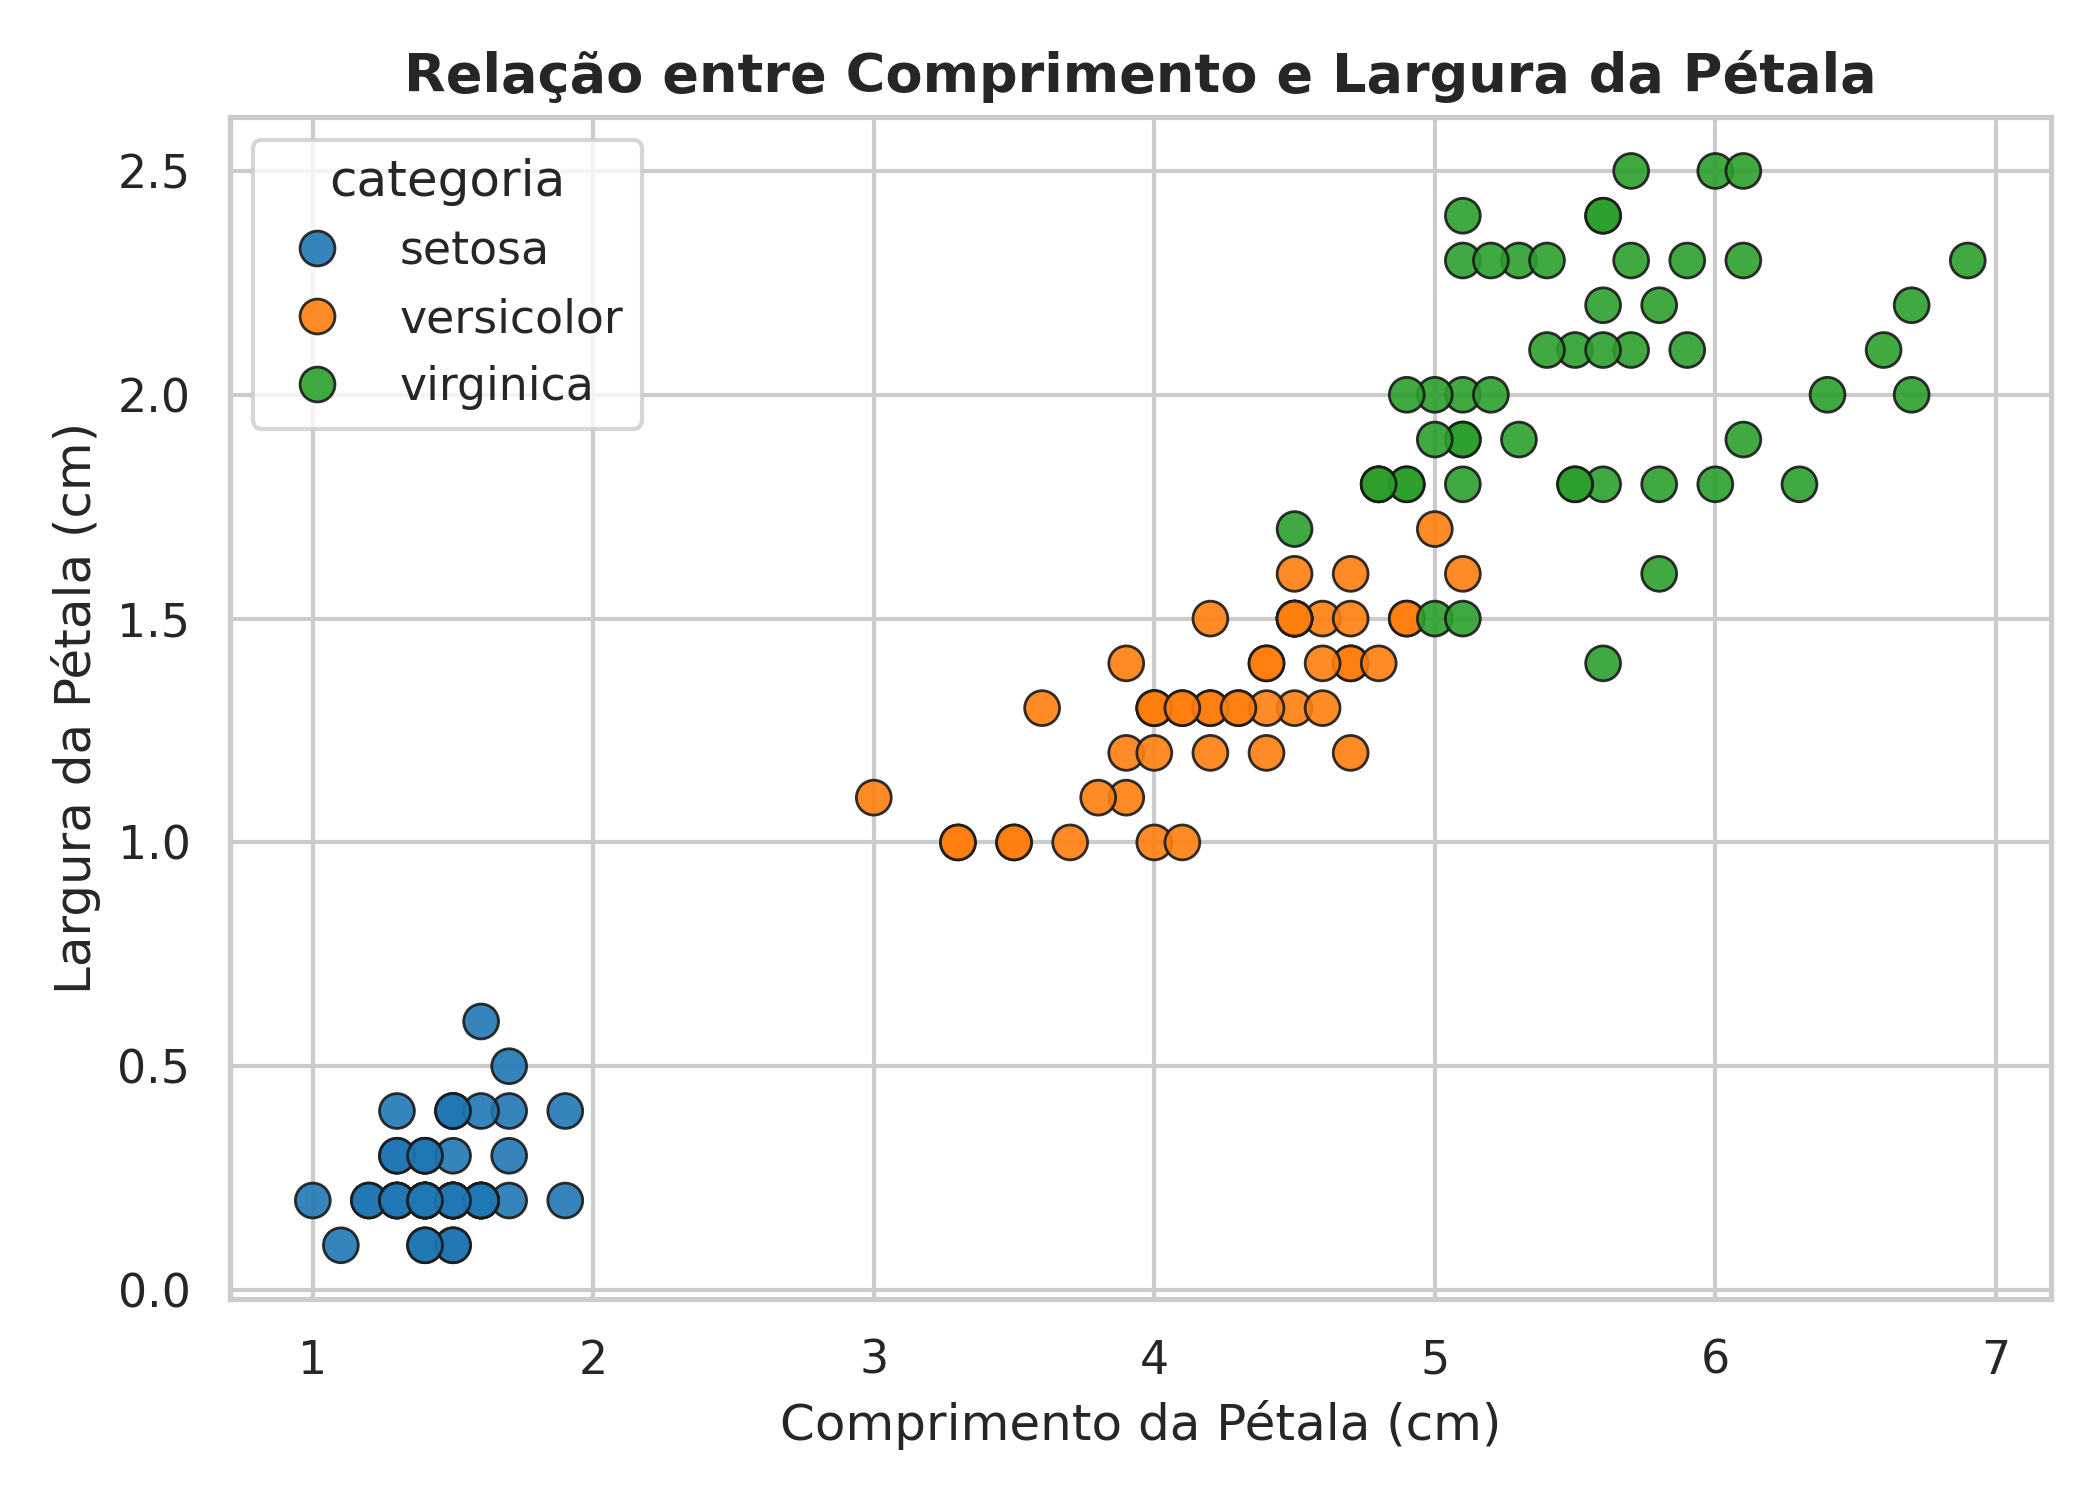
\includegraphics[width=0.88\columnwidth]{output/relacao_petala.png}
    \caption{Relação entre comprimento e largura da pétala por espécie.}
    \label{fig:petala}
\end{figure}

\subsection{Distribuição Tetradimensional}
A avaliação do \textit{pairplot} conjunto das 4 variáveis (Figura~\ref{fig:pairplot}) confirma que as dimensões das pétalas são as características mais determinantes para separar as classes, enquanto as medidas de sépala servem como suporte para o refinamento da fronteira entre \textit{Versicolor} e \textit{Virginica}.

\begin{figure}[!ht]
    \centering
    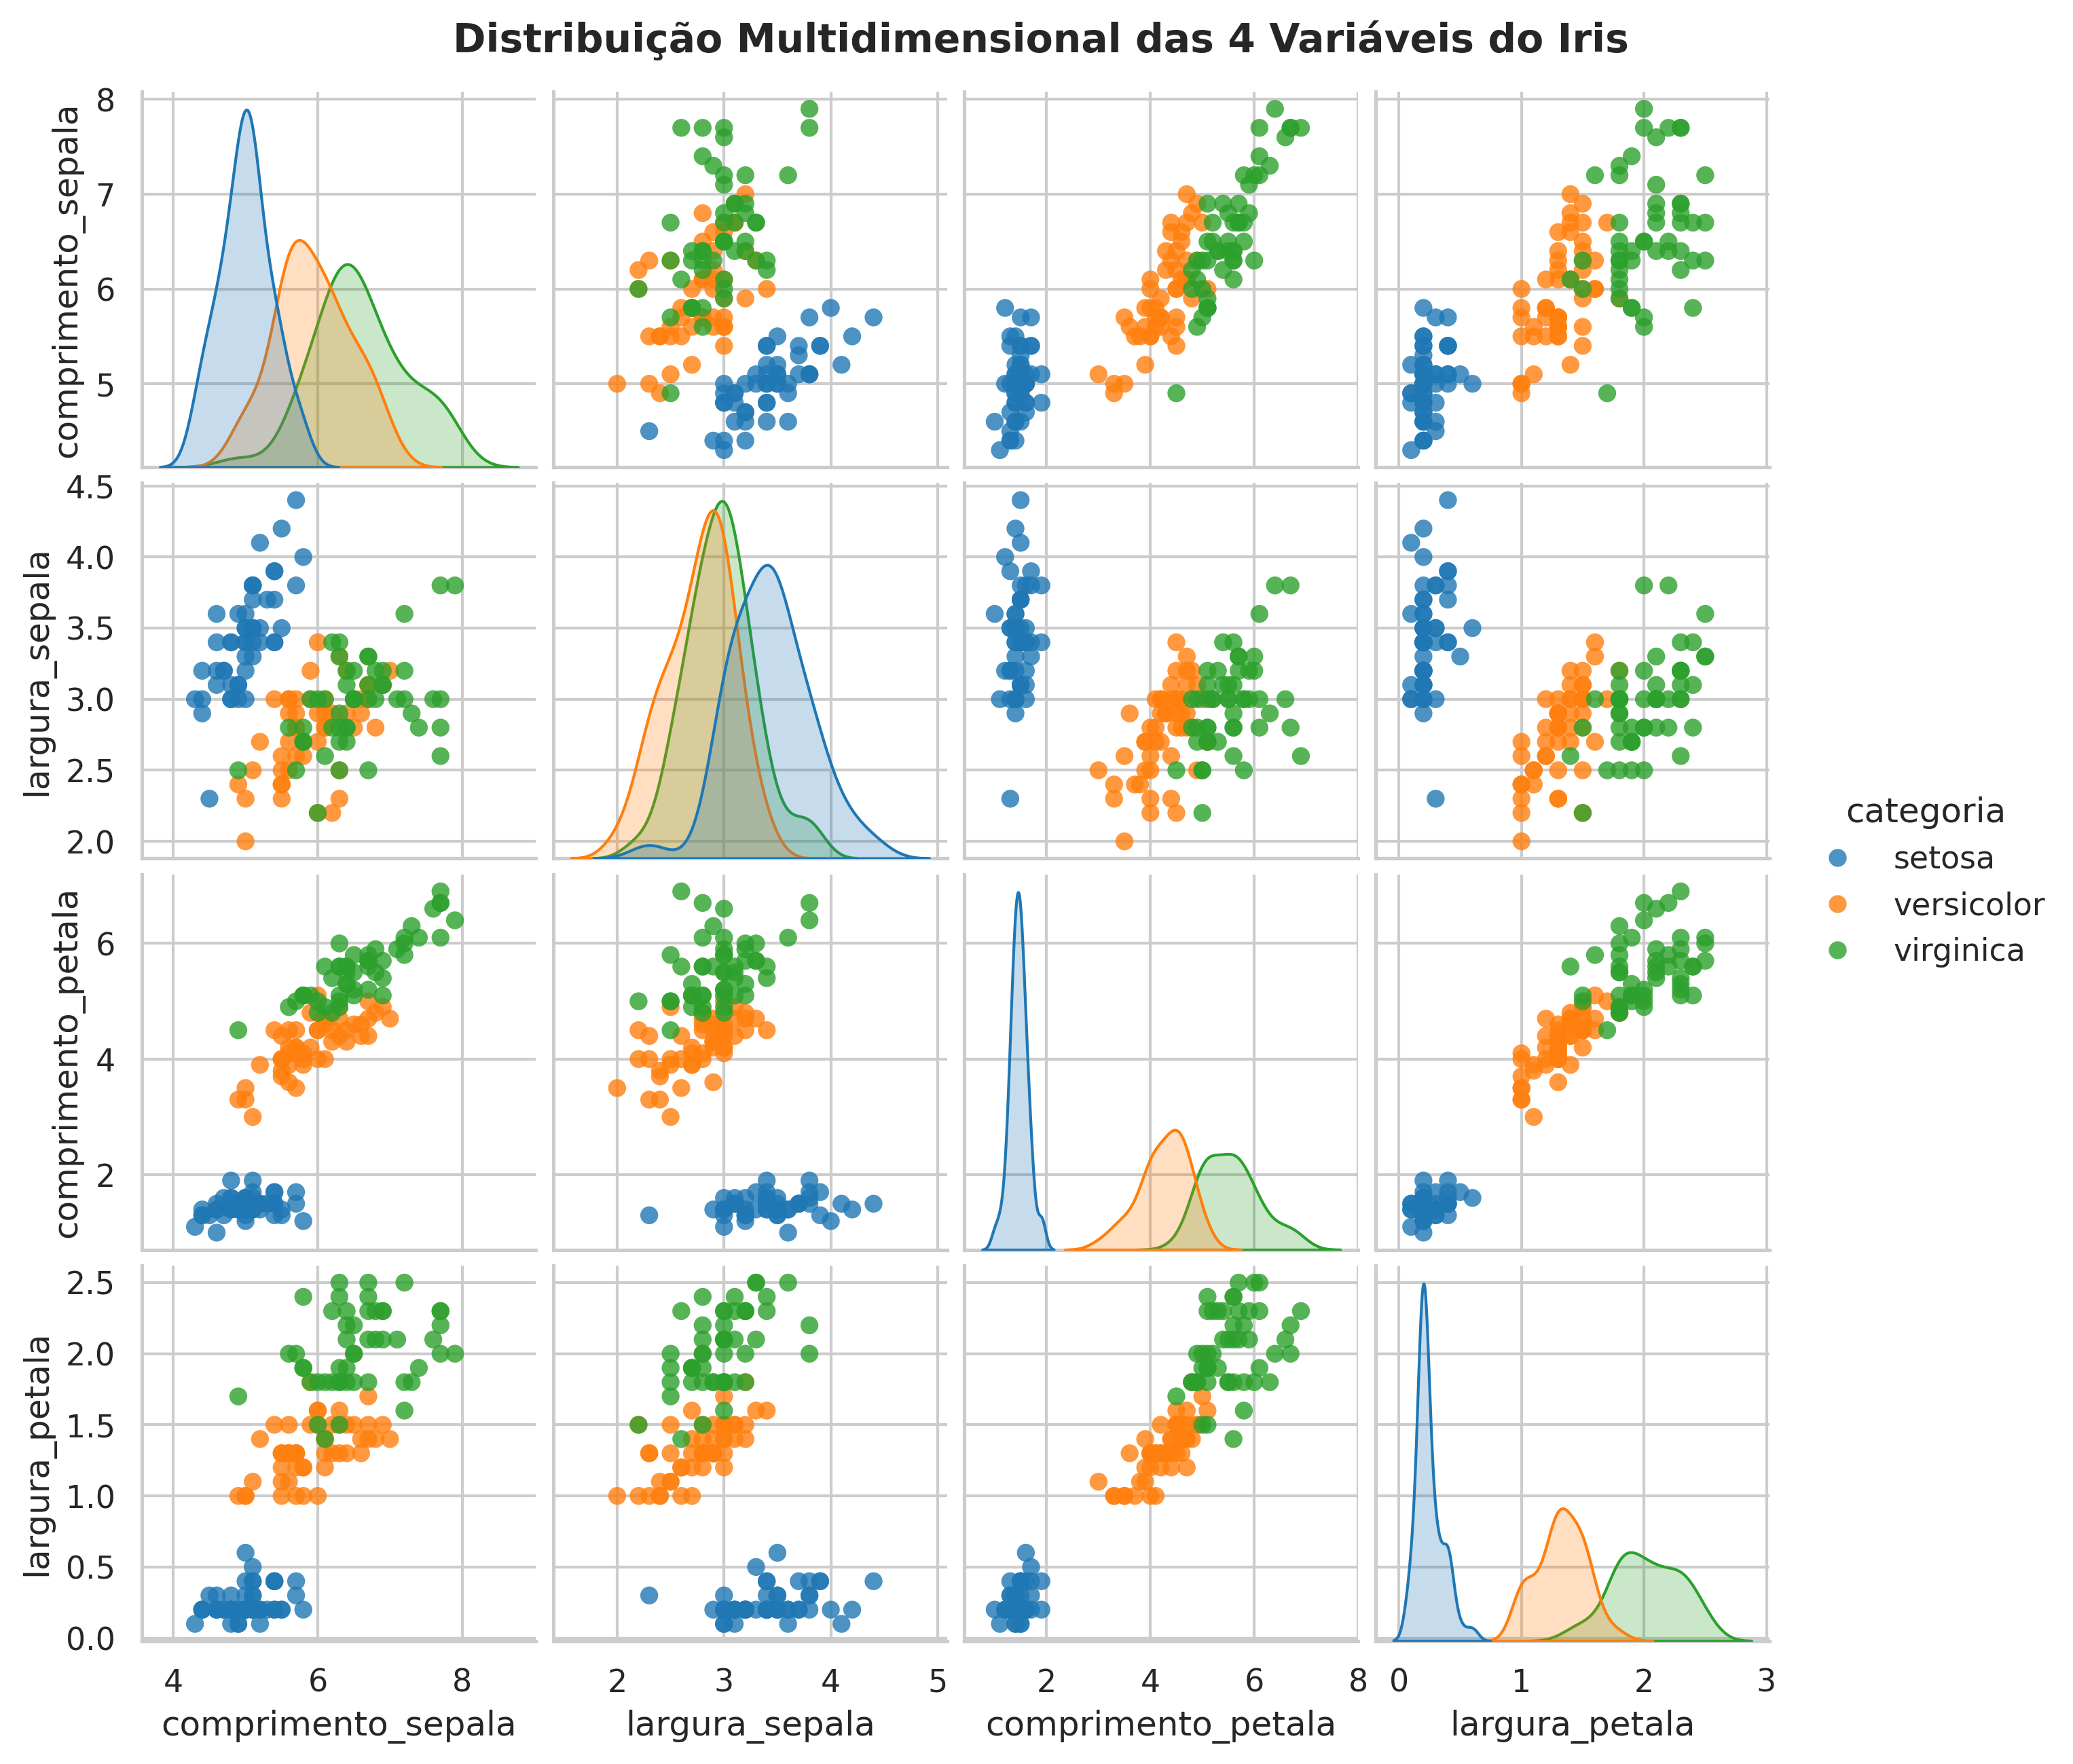
\includegraphics[width=\columnwidth]{output/distribuicao_4d_pairplot.png}
    \caption{Distribuição multidimensional (pairplot) das 4 variáveis.}
    \label{fig:pairplot}
\end{figure}

\section{Principal Component Analysis (PCA)}
Antes do PCA, as 4 variáveis foram padronizadas (média zero e variância unitária). O cálculo dos autovalores da matriz de covariância produziu os seguintes percentuais de variância explicada:
\begin{itemize}
    \item \textbf{PC1:} $72{,}96\%$
    \item \textbf{PC2:} $22{,}85\%$ (Acumulada: $95{,}81\%$)
    \item \textbf{PC3:} $3{,}67\%$ e \textbf{PC4:} $0{,}52\%$
\end{itemize}

Com apenas os dois primeiros componentes principais (PC1 e PC2), preserva-se praticamente toda a informação do espaço original ($95{,}81\%$). 

Na projeção 2D resultante (Figura~\ref{fig:pca}), a \textit{Setosa} aparece linearmente separável no lado esquerdo ($PC1 < -1$), refletindo seus altos coeficientes negativos em relação ao tamanho da pétala. Já \textit{Versicolor} e \textit{Virginica} dispõem-se ordenadamente ao longo do eixo horizontal, com mínima interseção de fronteira.

\begin{figure}[!ht]
    \centering
    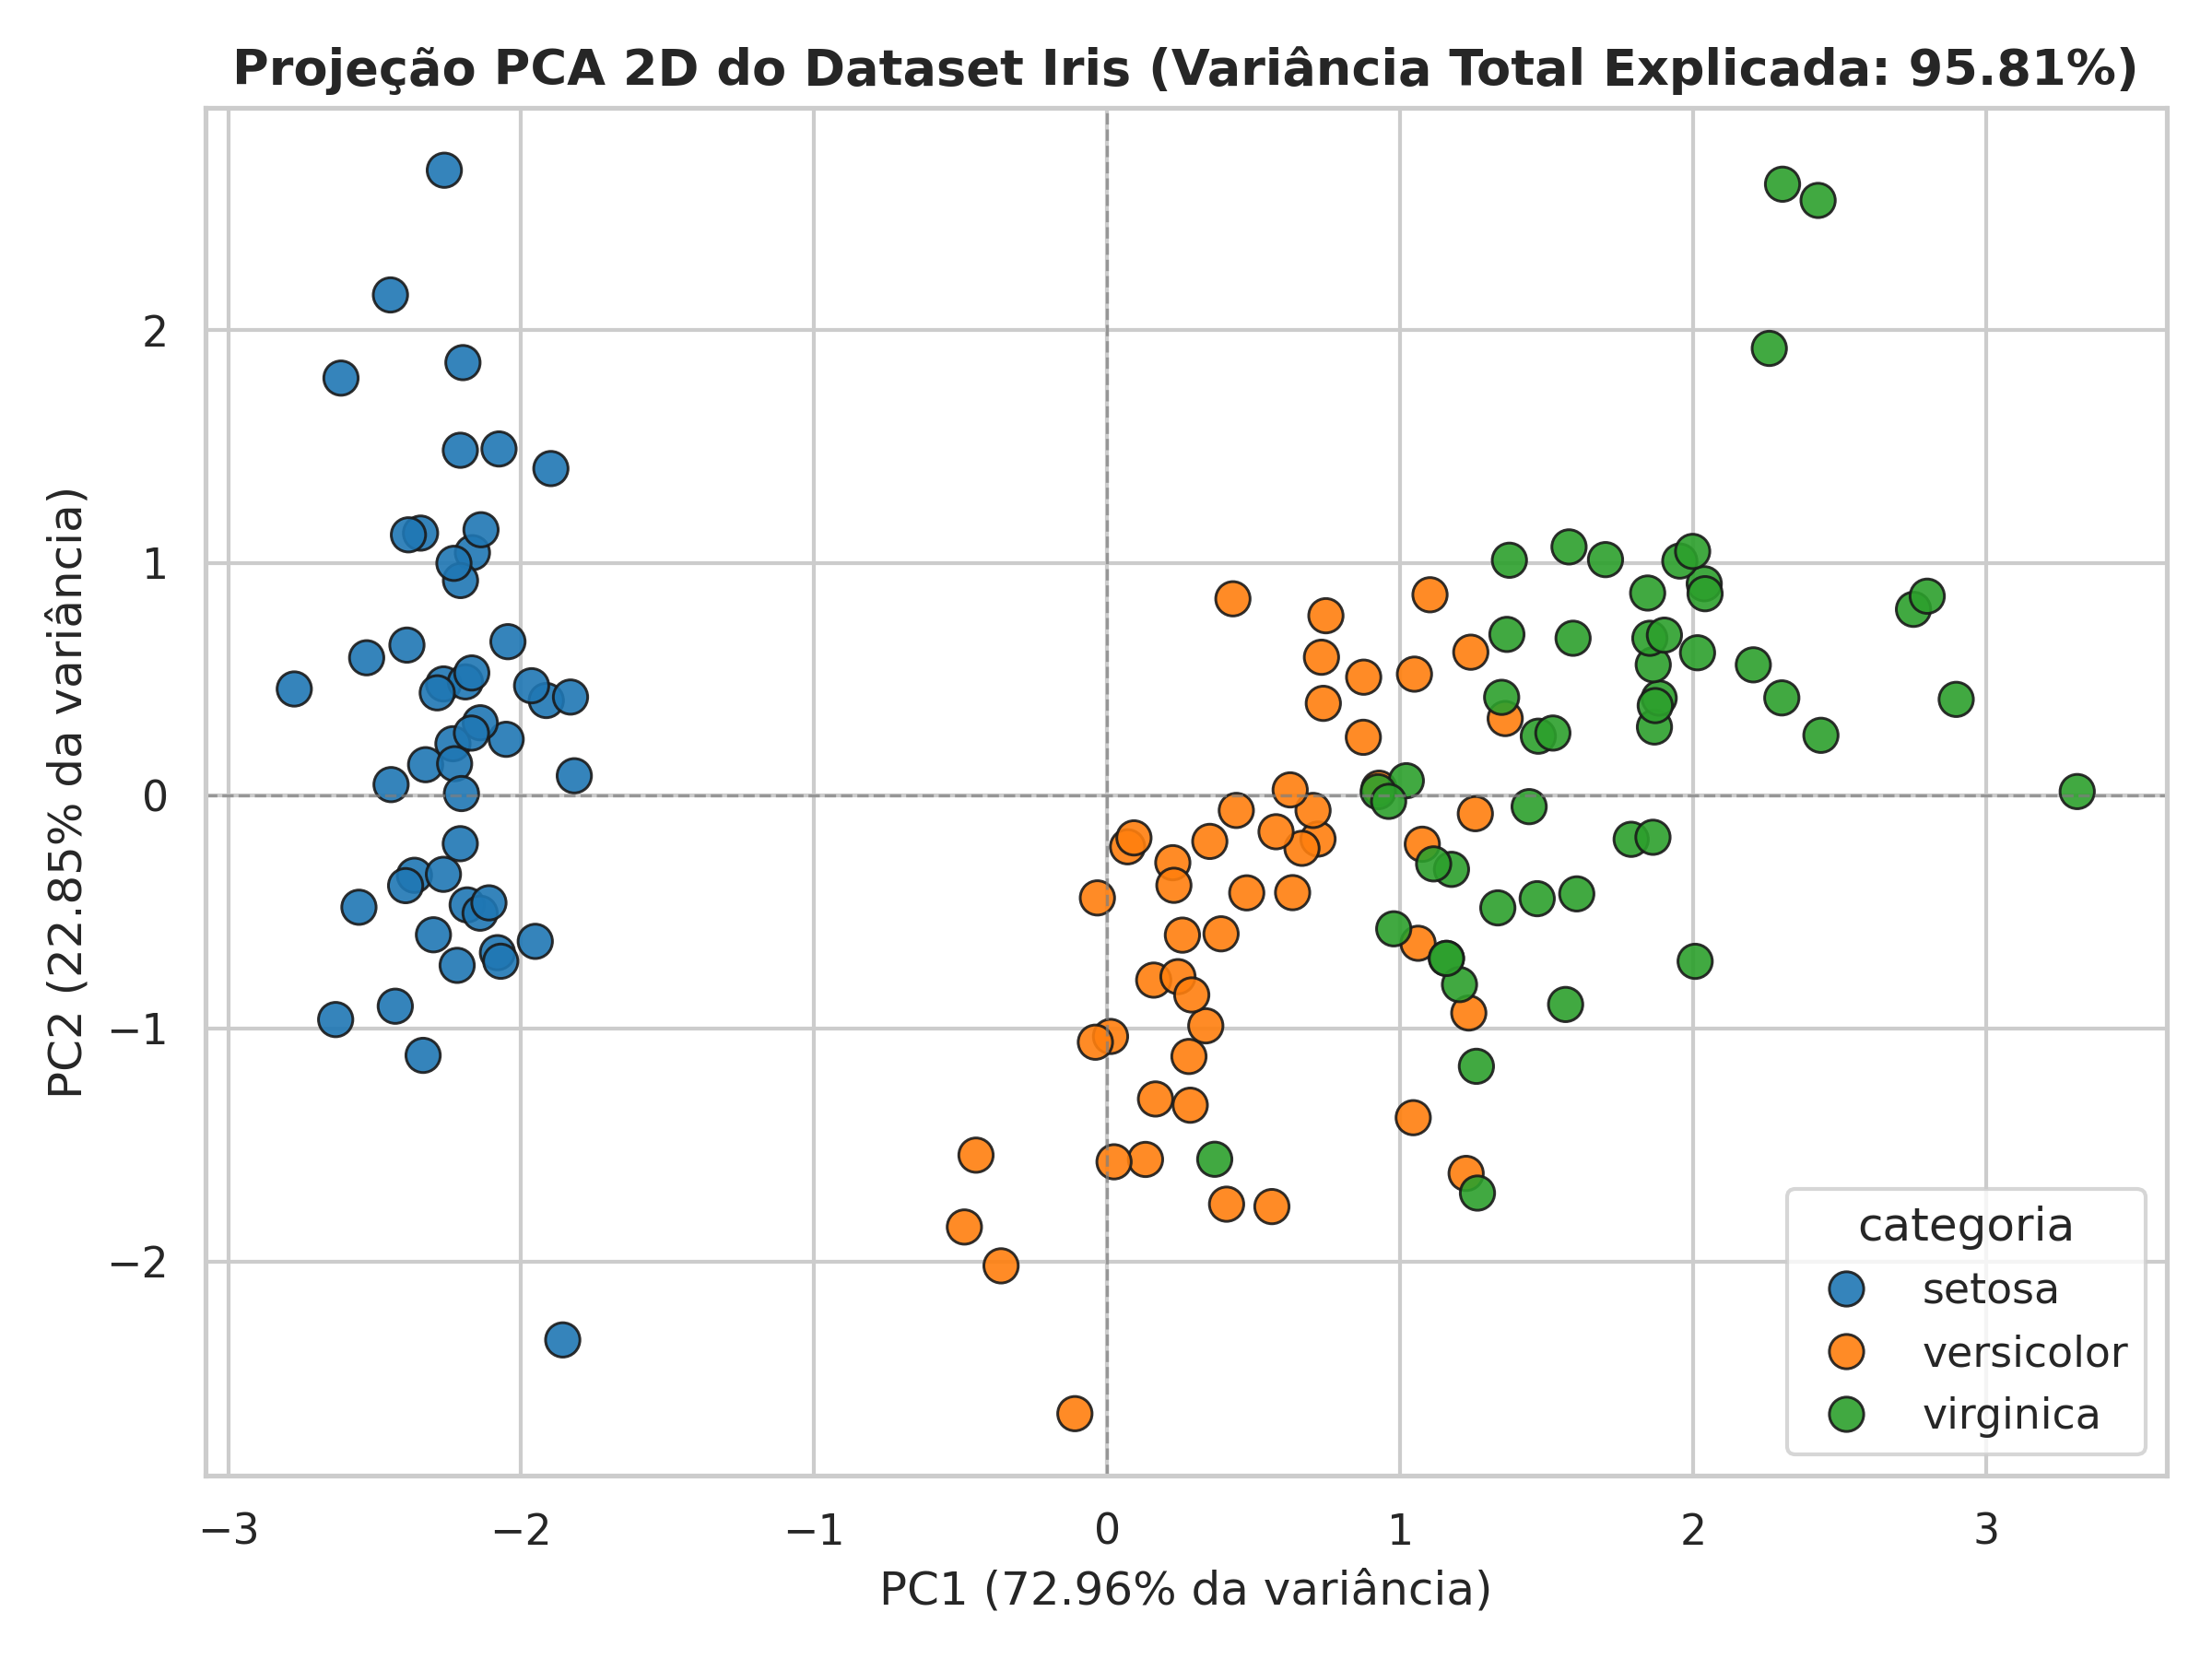
\includegraphics[width=0.88\columnwidth]{output/pca_2d.png}
    \caption{Projeção 2D do dataset Iris via PCA ($95{,}81\%$ da variância).}
    \label{fig:pca}
\end{figure}

\section{Classificação com K-NN}
O dataset foi dividido de forma estratificada em $80\%$ para treinamento (120 amostras) e $20\%$ para teste (30 amostras, 10 de cada classe), mantendo a semente aleatória (\texttt{random\_state=42}).

O classificador K-NN foi avaliado variando o número de vizinhos $K \in \{1, 3, 5, 7, 9, 11\}$:
\begin{itemize}
    \item Para $K=1, 7, 9, 11$: acurácia de \textbf{$96{,}67\%$} no teste 4D (apenas 1 erro em 30 amostras).
    \item Para $K=3$ e $K=5$: acurácia de \textbf{$93{,}33\%$} (2 erros entre \textit{Versicolor} e \textit{Virginica}).
    \item No espaço reduzido do PCA 2D, o modelo manteve acurácia de \textbf{$90{,}0\%$ a $93{,}33\%$}, confirmando que o PCA reteve quase toda a separabilidade discriminativa.
\end{itemize}

A Figura~\ref{fig:knn} ilustra as fronteiras de decisão geradas pelo K-NN no plano cartesiano dos dois componentes principais, mostrando regiões contínuas e bem delimitadas. A classe \textit{Setosa} obteve $100\%$ de precisão e revocação em todos os testes.

\begin{figure}[!ht]
    \centering
    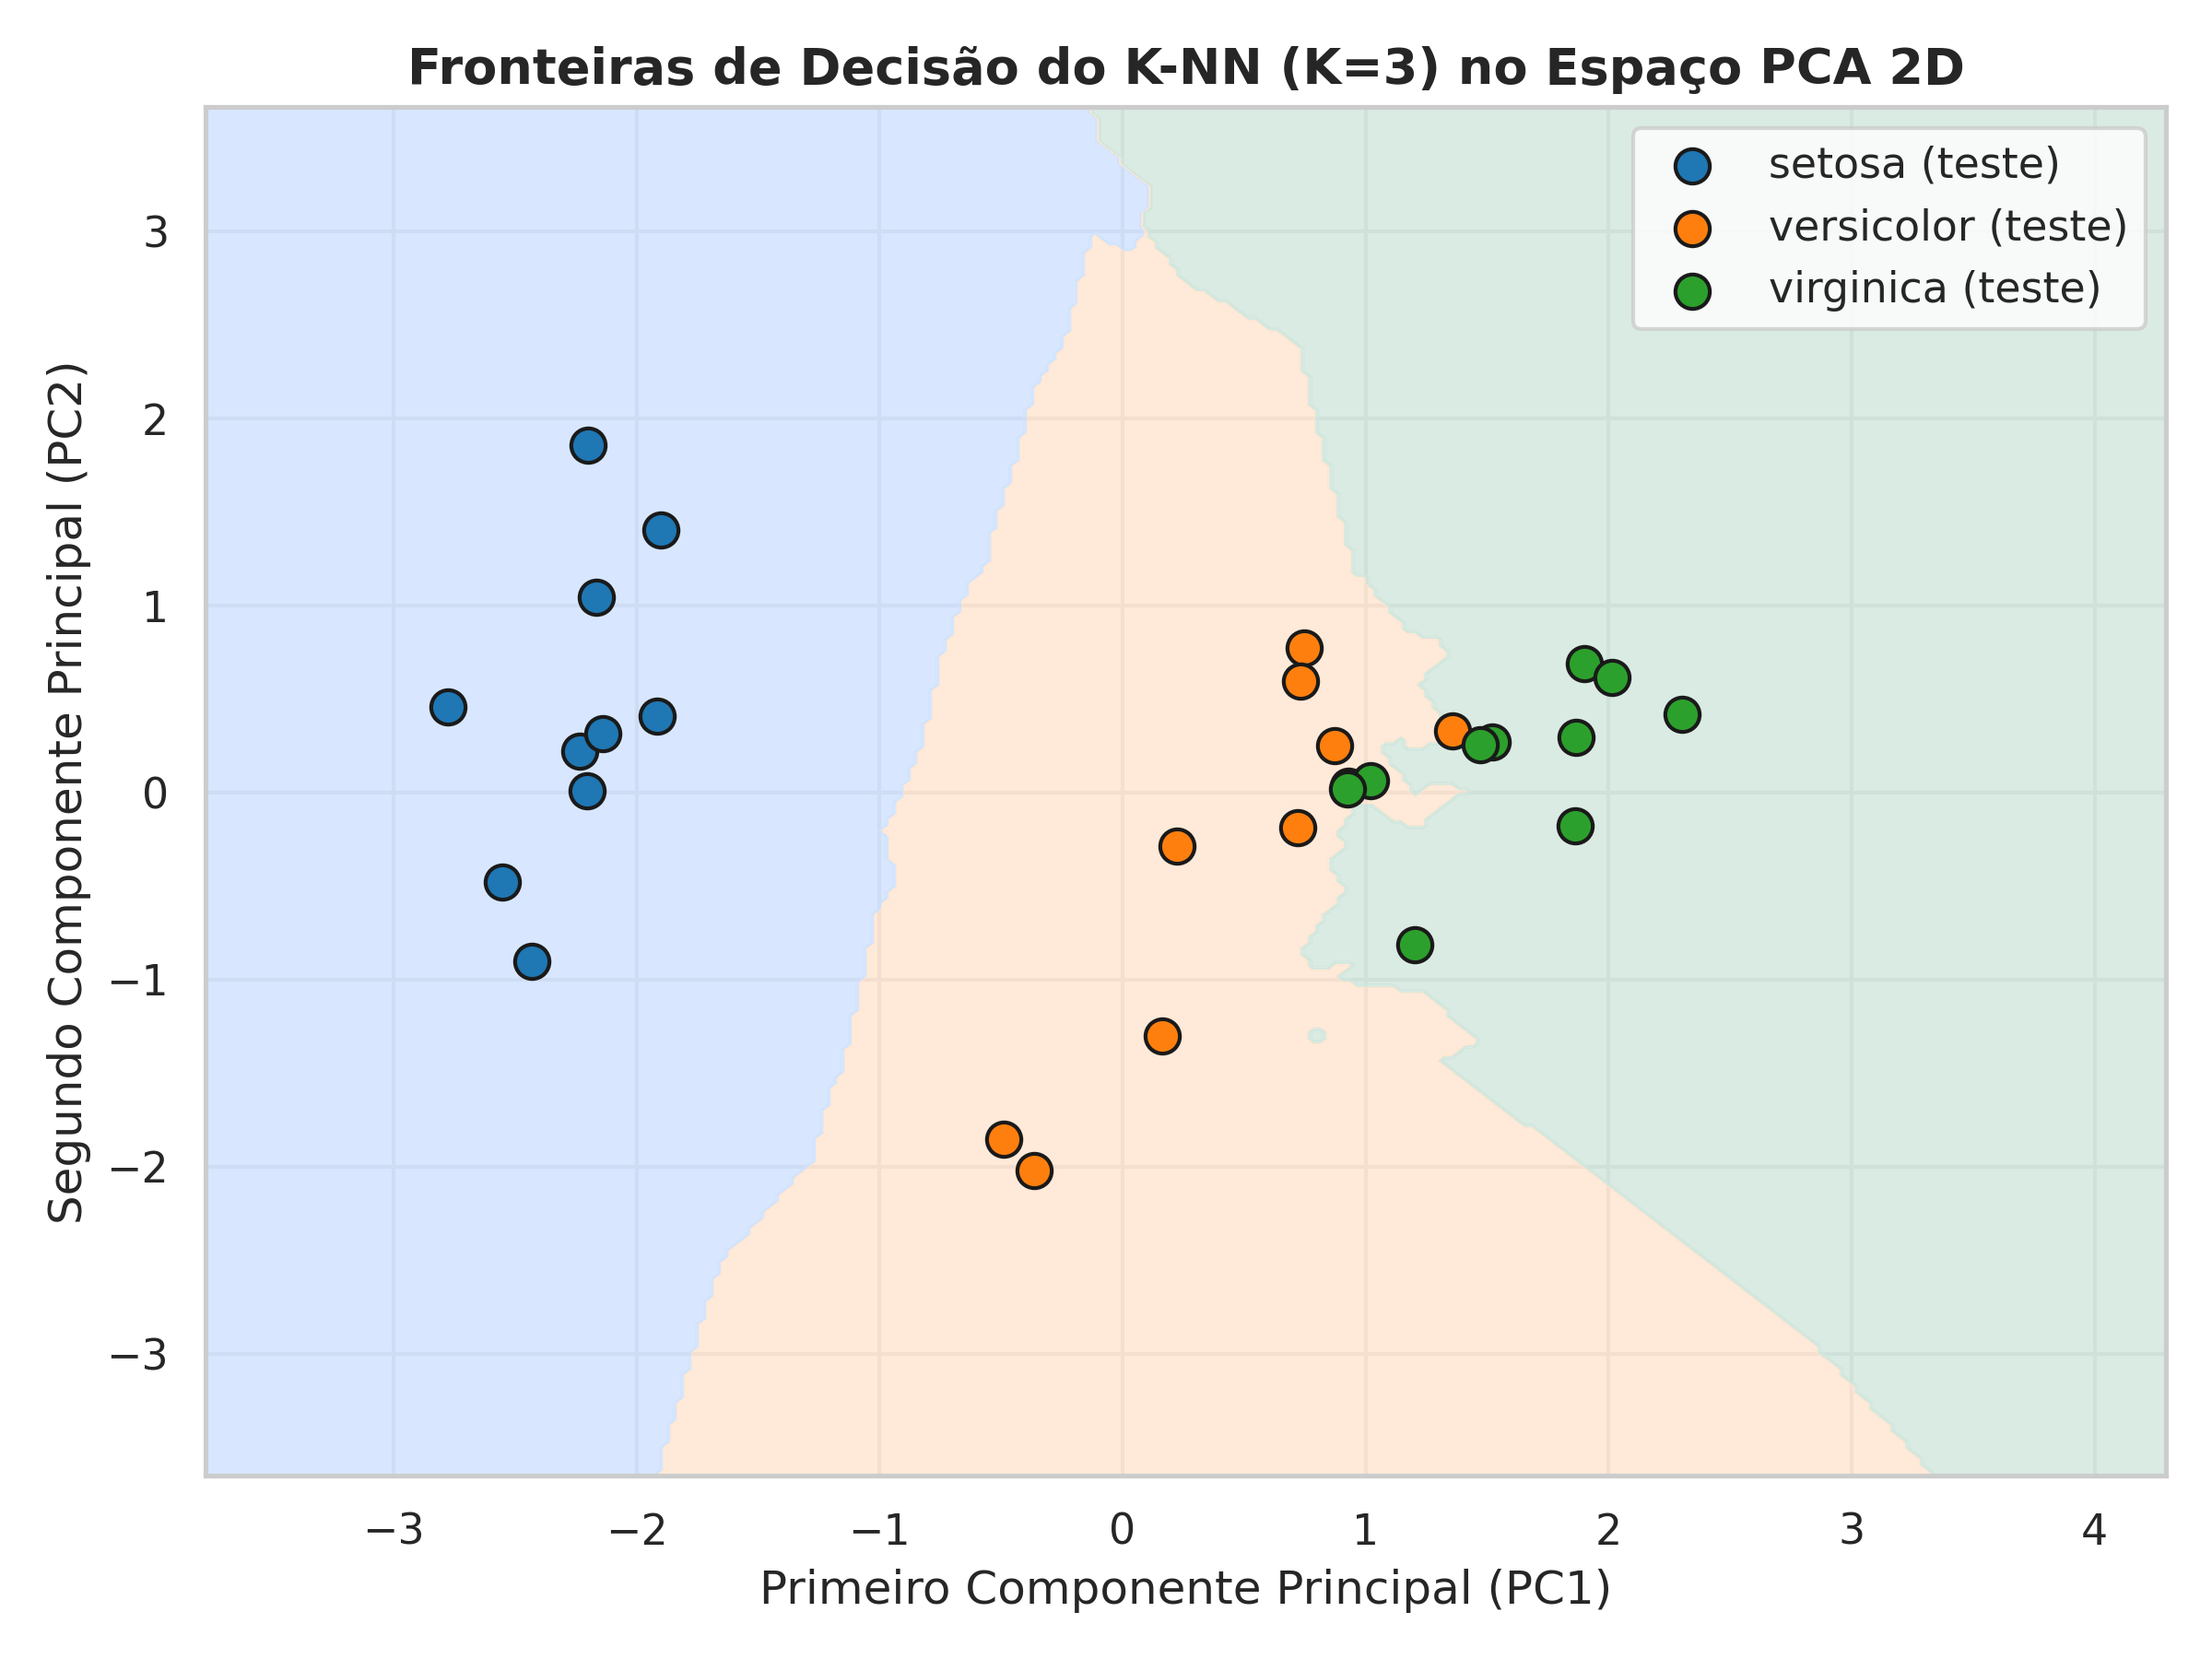
\includegraphics[width=0.88\columnwidth]{output/knn_fronteira_decisao.png}
    \caption{Fronteiras de decisão do K-NN no plano dos componentes principais.}
    \label{fig:knn}
\end{figure}

\section{Conclusão}
Os experimentos evidenciaram que o dataset Iris possui excelente estrutura geométrica para classificação. As dimensões de pétala são os atributos mais informativos, permitindo ao PCA condensar quatro variáveis em duas dimensões com $95{,}81\%$ de representatividade. O algoritmo K-NN comprovou alta eficácia prática, alcançando até $96{,}67\%$ de acurácia mesmo com uma amostragem compacta de teste.

\vspace{12pt}
\noindent\textbf{Link para o Código (Git):} \\
\url{https://github.com/JPeeeeee/visaoComputacional}

\end{document}
